\documentclass[a4paper,12pt]{article}
\usepackage{pdflscape, float, graphicx, color, listings, color}
\usepackage[top=1.5cm, bottom=1.6cm, left=2.0cm, right=2.0cm]{geometry}
\usepackage[dvipsnames]{xcolor}
\title{CS22510 Assignment 1\\
Runners and Riders\\
"Out and About"}
\author{Chris Savill\\\texttt{chs17@aber.ac.uk}}

\lstdefinestyle{customc++} {
  belowcaptionskip=1\baselineskip,
  breaklines=true,
  frame=L,
  language=C++,
  showstringspaces=false,
  basicstyle=\footnotesize\ttfamily,
  keywordstyle=\bfseries\color{OliveGreen},
  commentstyle=\itshape\color{black},
  identifierstyle=\color{blue},
  stringstyle=\color{orange},
  numbers=left
}

\lstdefinestyle{customjava} {
  belowcaptionskip=1\baselineskip,
  breaklines=true,
  frame=L,
  language=Java,
  showstringspaces=false,
  basicstyle=\footnotesize\ttfamily,
  keywordstyle=\bfseries\color{blue},
  commentstyle=\itshape\color{black},
  identifierstyle=\color{OliveGreen},
  stringstyle=\color{orange},
  numbers=left
}


\begin{document}
\maketitle
\newpage
\tableofcontents
\newpage

\section{Description of three programs}

\subsection{Event Creation Program}
\noindent Implemented in C++, this program was the simplest program to implement. Designing the program was quite easy as well due to how well this program suited an object oriented programming language such as C++. As the program was required to create an event with courses and competitors it made sense to make each of these a class with their related data members and member functions encapsulated together within their respective classes.

\vspace{5mm}
\noindent As the program's main purpose involved getting the user to input the details of the event, the courses, and the competitors, I decided to make the input processes robust by using checks and getting the user to double check their inputs. Although this may make the process long-winded I think the purpose they serve is worth the time. Another feature to improve robustness was to make sure that a user could not create a competitor without at least one course, otherwise competitors could be assigned a course that does not exist. With relation to assumptions, one assumption I made was that the tracks had no role in this program and that the tracks are generated/decided elsewhere once the courses have been created. This made generating the courses simpler as the only real checks needed were that valid nodes were selected and that the start and end nodes matched.

\subsection{Checkpoint Manager Program}
\noindent Implemented in Java this mainly GUI driven program took a bit of thinking with regards to the design. The main issue was figuring out how much information the program would require and the processing needed to validate a record. I made the assumption that records would arrive in chronological order to simplify the program and avoiding having to rewrite history. This meant that the program would only have to append to the time record file and only had to read in what it did not contain since it's last read.

\vspace{5mm}
\noindent With relation to making the program robust, I found it hard to cover every scenario that could be encountered so making the assumption that records would be entered in chronological order made things a lot easier. To make the program more robust I focused on the GUI design, keeping it simple and only supplying options to the user which would be easy to validate and reduce chances of error. By getting the type of checkpoint first, the program is able to filter the list of checkpoints in the next window thus getting rid of the user's need to check the type of checkpoint. Also there is a prompt telling the user they need to select both a checkpoint and competitor if only one was selected.

\vspace{5mm}
\noindent After getting the record details from the user I had to think about how to validate the new record and how to decide whether or not to append the new record to the time record file. I noticed that the program would need to keep track of every competitor's status and their current progress during the event. Using that information would allow the program to evaluate whether or not a new record is valid such as the program checking if the a competitor can be at a new checkpoint if the status tracked says that the competitor is currently at a medical checkpoint thus invalidating the new record.

\subsection{Event Manager Program}
\noindent Implemented in C this program did not require much work as I used the same program I implemented but removed the function to manually supply a time for a competitor and added the file locking capability to the accessing of the time record files and the implementation of writing a log file of the user's actions. As the program worked extremely well already I decided not to change any of the functionality just add the 2 new features and remove the 1 no longer needed.

\section{Code for the Event Creation Program}
\subsection{Header files}
\lstinputlisting[style=customc++, label={creator.h}, caption=Header file for non-class specific functions.]{"/home/clsavill/GitHub/Runners_and_Riders_3_Part/Event_Creation_Program/creator.h"}
\lstinputlisting[style=customc++, label={event.h}, caption=Header file Event class.]{/home/clsavill/GitHub/Runners_and_Riders_3_Part/Event_Creation_Program/event.h}
\lstinputlisting[style=customc++, label={course.h}, caption=Header file for Course class.]{/home/clsavill/GitHub/Runners_and_Riders_3_Part/Event_Creation_Program/course.h}
\lstinputlisting[style=customc++, label={competitor.h}, caption=Header file for Competitor class.]{/home/clsavill/GitHub/Runners_and_Riders_3_Part/Event_Creation_Program/competitor.h}

\subsection{Cpp files}
\lstinputlisting[style=customc++, label={creator.cpp}, caption=Main method and menu file.]{/home/clsavill/GitHub/Runners_and_Riders_3_Part/Event_Creation_Program/main.cpp}
\lstinputlisting[style=customc++, label={event.cpp}, caption=Cpp file for Event class.]{/home/clsavill/GitHub/Runners_and_Riders_3_Part/Event_Creation_Program/event.cpp}
\lstinputlisting[style=customc++, label={course.cpp}, caption=Cpp file for Course class.]{/home/clsavill/GitHub/Runners_and_Riders_3_Part/Event_Creation_Program/course.cpp}
\lstinputlisting[style=customc++, label={competitor.cpp}, caption=Cpp file for Competitor class.]{/home/clsavill/GitHub/Runners_and_Riders_3_Part/Event_Creation_Program/competitor.cpp}

\section{Clean build and compilation of Event Creation Program}
\lstinputlisting[breaklines=true, basicstyle=\footnotesize\ttfamily]{/home/clsavill/GitHub/Runners_and_Riders_3_Part/Event_Creation_Program/Event_Creation_Clean_And_Build_Log.txt}

\section{Run through of Event Creation Program}
\lstinputlisting[breaklines=true, basicstyle=\footnotesize\ttfamily]{/home/clsavill/GitHub/Runners_and_Riders_3_Part/Event_Creation_Program/Event_Creation_Runthrough.txt}

\section{Files created by execution of Event Creation Program}
\lstinputlisting[breaklines=true, basicstyle=\footnotesize\ttfamily, caption=Event 'name.txt' file]
{/home/clsavill/GitHub/Runners_and_Riders_3_Part/Event_Creation_Program/name.txt}

\lstinputlisting[breaklines=true, basicstyle=\footnotesize\ttfamily, caption=Event 'courses.txt' file]
{/home/clsavill/GitHub/Runners_and_Riders_3_Part/Event_Creation_Program/courses.txt}

\lstinputlisting[breaklines=true, basicstyle=\footnotesize\ttfamily, caption=Event 'entrants.txt' file]
{/home/clsavill/GitHub/Runners_and_Riders_3_Part/Event_Creation_Program/entrants.txt}

\section{Code for Checkpoint Manager Program}
\lstinputlisting[style=customjava, label={Launcher.java}, caption=Launcher class.]{/home/clsavill/GitHub/Runners_and_Riders_3_Part/Checkpoint_Manager_Program/src/Data_Structures/Launcher.java}
\lstinputlisting[style=customjava, label={Event.java}, caption=Event class.]{/home/clsavill/GitHub/Runners_and_Riders_3_Part/Checkpoint_Manager_Program/src/Data_Structures/Event.java}
\lstinputlisting[style=customjava, label={Node.java}, caption=Node class.]{/home/clsavill/GitHub/Runners_and_Riders_3_Part/Checkpoint_Manager_Program/src/Data_Structures/Node.java}
\lstinputlisting[style=customjava, label={Course.java}, caption=Course class.]{/home/clsavill/GitHub/Runners_and_Riders_3_Part/Checkpoint_Manager_Program/src/Data_Structures/Course.java}
\lstinputlisting[style=customjava, label={Competitor.java}, caption=Competitor class.]{/home/clsavill/GitHub/Runners_and_Riders_3_Part/Checkpoint_Manager_Program/src/Data_Structures/Competitor.java}
\lstinputlisting[style=customjava, label={Record.java}, caption=Record class.]{/home/clsavill/GitHub/Runners_and_Riders_3_Part/Checkpoint_Manager_Program/src/Data_Structures/Record.java}
\lstinputlisting[style=customjava, label={FileHandler.java}, caption=FileHandler class.]{/home/clsavill/GitHub/Runners_and_Riders_3_Part/Checkpoint_Manager_Program/src/File_Handling/FileHandler.java}
\lstinputlisting[style=customjava, label={TypeWindow.java}, caption=TypeWindow class.]{/home/clsavill/GitHub/Runners_and_Riders_3_Part/Checkpoint_Manager_Program/src/GUI/TypeWindow.java}
\lstinputlisting[style=customjava, label={SelectionWindow.java}, caption=SelectionWindow class.]{/home/clsavill/GitHub/Runners_and_Riders_3_Part/Checkpoint_Manager_Program/src/GUI/SelectionWindow.java}
\lstinputlisting[style=customjava, label={TimeWindow.java}, caption=TimeWindow class.]{/home/clsavill/GitHub/Runners_and_Riders_3_Part/Checkpoint_Manager_Program/src/GUI/TimeWindow.java}

\section{Clean build and compilation of Checkpoint Program}
\lstinputlisting[breaklines=true, basicstyle=\footnotesize\ttfamily]{/home/clsavill/GitHub/Runners_and_Riders_3_Part/Checkpoint_Manager_Program/Checkpoint_Manager_Clean_And_Build_Log.txt}

\section{Run through of Checkpoint Manager Program}
\begin{figure}[H]
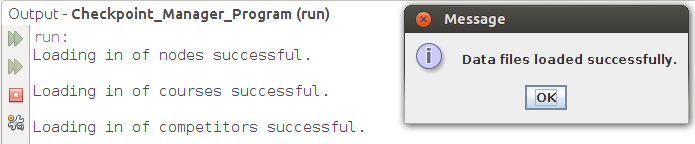
\includegraphics[scale=0.8]{/home/clsavill/GitHub/Runners_and_Riders_3_Part/Checkpoint_Manager_Program/CMP1.png}
\caption{Start up of GUI letting user know data file loaded successfully ( if they did) else the program would close.}
\end{figure}

\begin{figure}[H]
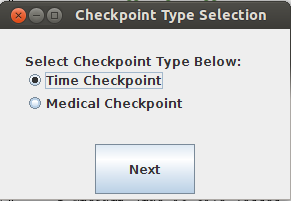
\includegraphics[scale=0.8]{/home/clsavill/GitHub/Runners_and_Riders_3_Part/Checkpoint_Manager_Program/CMP2.png}
\caption{Checkpoint type selection window showing the time checkpoint type selected.}
\end{figure}

\begin{figure}[H]
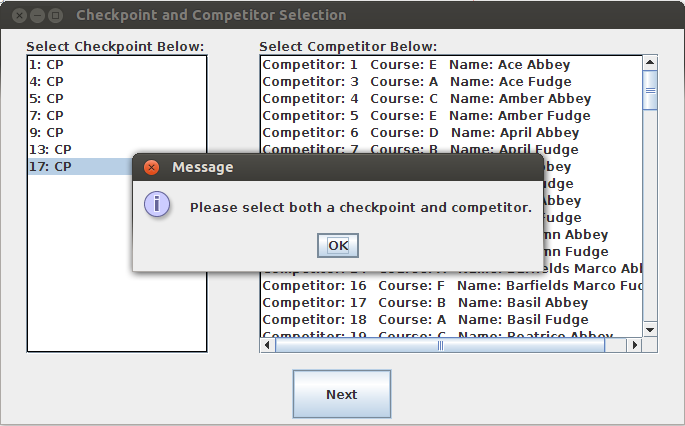
\includegraphics[scale=0.8]{/home/clsavill/GitHub/Runners_and_Riders_3_Part/Checkpoint_Manager_Program/CMP3.png}
\caption{Message that pops up when both a checkpoint and competitor are not selected.}
\end{figure}

\begin{figure}[H]
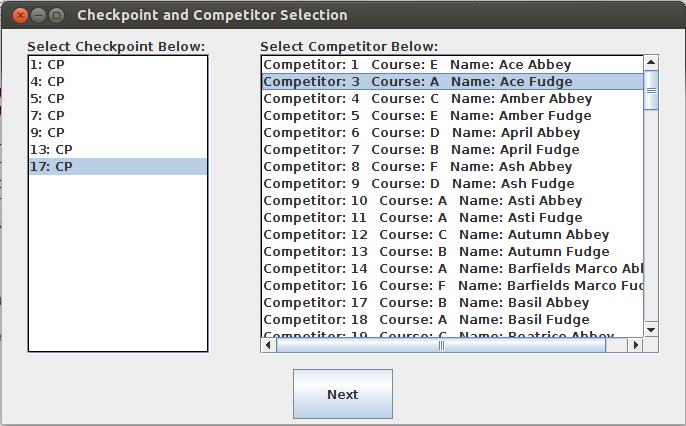
\includegraphics[scale=0.8]{/home/clsavill/GitHub/Runners_and_Riders_3_Part/Checkpoint_Manager_Program/CMP4.png}
\caption{Time checkpoint 17 selection and competitor 3 selected within selection window.}
\end{figure}

\begin{figure}[H]
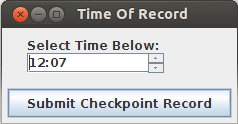
\includegraphics[scale=0.8]{/home/clsavill/GitHub/Runners_and_Riders_3_Part/Checkpoint_Manager_Program/CMP5.png}
\caption{Time window where the user has to input the time for the new record.}
\end{figure}

\begin{figure}[H]
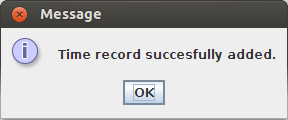
\includegraphics[scale=0.8]{/home/clsavill/GitHub/Runners_and_Riders_3_Part/Checkpoint_Manager_Program/CMP6.png}
\caption{Message stating that the new record was successfully added and written to the time records file.}
\end{figure}

\begin{figure}[H]
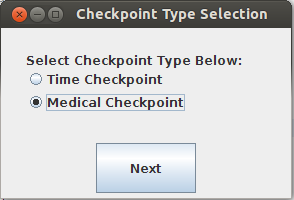
\includegraphics[scale=0.8]{/home/clsavill/GitHub/Runners_and_Riders_3_Part/Checkpoint_Manager_Program/CMP7.png}
\caption{Checkpoint type selection window showing the medical checkpoint type selected.}
\end{figure}

\begin{figure}[H]
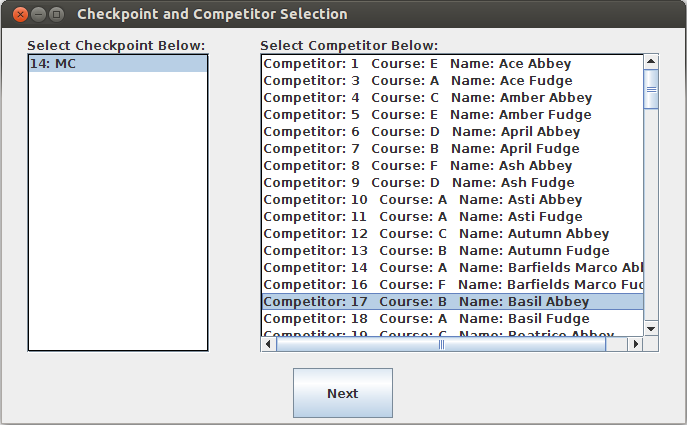
\includegraphics[scale=0.8]{/home/clsavill/GitHub/Runners_and_Riders_3_Part/Checkpoint_Manager_Program/CMP8.png}
\caption{Medical checkpoint 14 selection and competitor 17 selected within the selection window.}
\end{figure}

\begin{figure}[H]
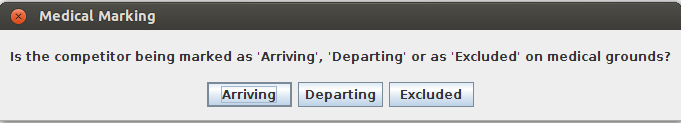
\includegraphics[scale=0.8]{/home/clsavill/GitHub/Runners_and_Riders_3_Part/Checkpoint_Manager_Program/CMP9.png}
\caption{Prompt asking the user the status of the competitor at the chosen medical checkpoint.}
\end{figure}

\begin{figure}[H]
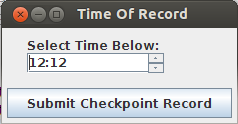
\includegraphics[scale=0.8]{/home/clsavill/GitHub/Runners_and_Riders_3_Part/Checkpoint_Manager_Program/CMP10.png}
\caption{Time window with a valid time entered (a time after the last record time.}
\end{figure}

\begin{figure}[H]
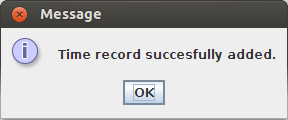
\includegraphics[scale=0.8]{/home/clsavill/GitHub/Runners_and_Riders_3_Part/Checkpoint_Manager_Program/CMP6.png}
\caption{Message stating that the new record was successfully added and written to the time records file.}
\end{figure}

\begin{figure}[H]
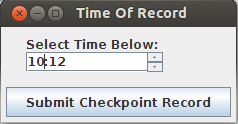
\includegraphics[scale=0.8]{/home/clsavill/GitHub/Runners_and_Riders_3_Part/Checkpoint_Manager_Program/CMP11.png}
\caption{The same record as above time window with an invalid time entered (a time before the last record time.}
\end{figure}

\begin{figure}[H]
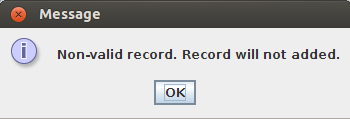
\includegraphics[scale=0.8]{/home/clsavill/GitHub/Runners_and_Riders_3_Part/Checkpoint_Manager_Program/CMP12.png}
\caption{Message stating that the new record attempted to be added was invalid (either the time was before the last record, or the system determined that the status given cannot be correct due to the current status of the competitor.}
\end{figure}

\section{Files created by execution of Checkpoint Manager\\Program}
\lstinputlisting[breaklines=true, basicstyle=\footnotesize\ttfamily, caption=Copy of cp\_times\_1.txt file from event\_3 that was read into the program plus 2 new records appended.]{/home/clsavill/GitHub/Runners_and_Riders_3_Part/Checkpoint_Manager_Program/cp_times.txt}

\section{Clean build and compilation of Event Manager Program}
\lstinputlisting[breaklines=true, basicstyle=\footnotesize\ttfamily]{/home/clsavill/GitHub/Runners_and_Riders_3_Part/Event_Manager_Program/Event_Manager_Clean_And_Build_Log.txt}

\begin{landscape}
\section{Run through of Event Manager Program}
\lstinputlisting[breaklines=true, basicstyle=\footnotesize\ttfamily]{/home/clsavill/GitHub/Runners_and_Riders_3_Part/Event_Manager_Program/Event_Manager_Runthrough.txt}

\section{Results list produced at the end of an event}

\subsection{Results of successful competitors}
\lstinputlisting[breaklines=true, basicstyle=\footnotesize\ttfamily]{/home/clsavill/GitHub/Runners_and_Riders_3_Part/Event_Manager_Program/Event_Manager_Results.txt}

\subsection{Table of excluded competitors}
\lstinputlisting[breaklines=true, basicstyle=\footnotesize\ttfamily]{/home/clsavill/GitHub/Runners_and_Riders_3_Part/Event_Manager_Program/Event_Manager_Excluded.txt}

\section{Log file contents}
\lstinputlisting[breaklines=true, basicstyle=\footnotesize\ttfamily]{/home/clsavill/GitHub/Runners_and_Riders_3_Part/Event_Manager_Program/log.txt}

\end{landscape}

\end{document}